\subsection{Malware Behaviors}
\label{sec:profile:behavior}

Table~\ref{table:behavior} illustrates the behaviors of
malware families\footnote{Table~\ref{table:behavior} aggregates the behaviors over
all malware varieties in a family. The more specific per-variety breakdown can be found 
at our \amd.} we analyzed.
Due to space constraint we only present part of the analysis result. The
more detailed information can be found at our \amd. Behavior tags in one
category may not be mutually-exclusive --- some apps may present multiple behaviors
in a category.

\begin{table*}[!t]
\centering
\caption{Malware Behaviors.}
\label{table:behavior}
\begin{subtable}{1\textwidth}
\centering
\scriptsize
\resizebox{\textwidth}{!}{ %
\begin{tabular}{|l|l|l|l|l|l|l|l|}
\hline
\multicolumn{8}{|c|}{{\bf Legend}} \\
\hline
{\bf Composition} & Standalone (ST) & \multicolumn{2}{l|}{Repackaging (RPKG): Isolated (O), Integrated (T)} & Library (LIB) & {\bf Installation} & Drop (DR) & Drive-by Download (DD) \\
\hline
{\bf Activation}  & Event (EV) & \multicolumn{2}{l|}{By Host App (BHA)} & Scheduling (SC) & {\bf Info Stealing} & Device Info (DI) & Personal Info (PI) \\
\hline
\multirow{2}{*}{\bf Persistence} & \multicolumn{1}{l}{Stealthy (TH):} & \multicolumn{6}{l|}{Block (BL), Clean (CL), Hide Icon (HI), Rootkit (RK)} \\
\cline{2-8}
                                                  &  \multicolumn{1}{l}{Prevent destroy (PD):} & \multicolumn{6}{l|}{Hide Admin (HA), Kill AV (KA), Lock Device (LD), Monitor Destroy Action (MDA), Reinstall (RI), System App (SYS)} \\
\cline{1-8}
{\bf Privilege} & Request Admin (RA) & \multicolumn{6}{l|}{Root Exploit (RE)} \\
\hline
{\bf C\&C} & Internet (IN) & \multicolumn{6}{l|}{Command Encoding (CE): JSON (J), Java Script (JS), XML (X), Custom Protocol (P)} \\
\hline
\multirow{2}{*}{\bf Anti-analysis}  & Renaming (RN) & String Encryption (SE) & Dynamic Loading (DL) & \multicolumn{4}{l|}{Native Payload (NP)} \\
\cline{2-8}
                              & \multicolumn{7}{l|}{Evade Dynamic Analysis (EDA): Check Device Info (CDI), Encrypt Communication (EC), Check Installed App (CIA)} \\
\hline
\end{tabular}
}
\end{subtable}%

\begin{subtable}{1\textwidth}
\centering
\scriptsize
\resizebox{1\textwidth}{!}{ %
\begin{tabular}{?p{2.3cm}?c|c|c?c|c?c|c|c?c|c?c|c?c|c?c|c|c?c|c|c|c|c?}
\Xhline{2\arrayrulewidth}
\multirow{2}{*}{Family} & \multicolumn{3}{c?}{Composition} & \multicolumn{2}{c?}{Installation} & \multicolumn{3}{c?}{Activation} & \multicolumn{2}{c?}{Info Stealing} & \multicolumn{2}{c?}{Persistence} & \multicolumn{2}{c?}{Privilege} & \multicolumn{3}{c?}{C\&C} & \multicolumn{5}{c?}{Anti-analysis} \\
\cline{2-23}
 & ST & RPKG & LIB  & DR & DD & EV & BHA & SC & DI & PI & TH & PD & RA & RE & IN & SMS & CE & RN & SE & DL & NP & EDA \\
\hline
\hline
Airpush &  &  & \checkmark  &  &  &  & \checkmark & \checkmark & \checkmark & \checkmark &  &  &  & & \checkmark &  & J & \checkmark &  &  &  &  \\
\hline
AndroRAT & \checkmark & & & \checkmark &  & \checkmark &  & \checkmark & \checkmark & \checkmark &  &  &  & & \checkmark &  & P &  &  &  &  & \\
\hline
Andup &  &  & \checkmark & \checkmark &  & \checkmark & \checkmark &  & \checkmark &  &  &  &  & &  &  &  & \checkmark & \checkmark &  &  &  \\
\hline
Aples & \checkmark &  &  &  &  & \checkmark &  & \checkmark & \checkmark &  &  & LD & \checkmark & & \checkmark &  & P &  &  &  &  & \\
\hline
BankBot & \checkmark & &   & \checkmark & \checkmark & \checkmark &  & \checkmark & \checkmark & \checkmark & BL\&HI & MDA & \checkmark & & \checkmark & \checkmark & J\&P & \checkmark & \checkmark & \checkmark &  & CDI \\
\hline
Bankun & \checkmark & &   & \checkmark & \checkmark & \checkmark &  & \checkmark & \checkmark & \checkmark & BL\&HI &  & \checkmark & & \checkmark &  & J\&X &  &  &  &  & CDI \\
\hline
Boqx &  & O &  & \checkmark &  & \checkmark &  &  &  &  &  &  &  & &  &  &  &  &  &  & \checkmark &  \\
\hline
Boxer & \checkmark & &   &  & \checkmark & \checkmark &  &  &  &  &  &  &  & &  &  &  & \checkmark & \checkmark &  &  &  \\
\hline
Cova & \checkmark &  &  & \checkmark &  & \checkmark &  &  & \checkmark & \checkmark & BL &  &  &  & \checkmark &  & JS & \checkmark &  &  &  &  \\
\hline
Dowgin &  & & \checkmark & \checkmark &  & \checkmark & \checkmark &  & \checkmark &  &  &  &  & & \checkmark &  & J & \checkmark & \checkmark & \checkmark &  & EC \\
\hline
DroidKungFu & \checkmark & O\&T &   & \checkmark &  & \checkmark & \checkmark & \checkmark & \checkmark & \checkmark &  & KA &  & \checkmark & \checkmark &  & J\&P & \checkmark & \checkmark &  & \checkmark & \\
\hline
Erop & \checkmark &  &  &  &  & \checkmark &  &  & \checkmark &  &  &  &  &   &  &  &  &  &  &  &  &  \\
\hline
FakeAV & \checkmark & &   &  &  & \checkmark &  & \checkmark &  &  & BL &  &  & &  &  &  &  &  &  &  &   \\
\hline
FakeAngry &  & O &   & \checkmark &  & \checkmark &  &  & \checkmark &  &  &  &  & & \checkmark &  & P & \checkmark & \checkmark &  &  & \\
\hline
FakeDoc & \checkmark &  &  &  &  & \checkmark &  & \checkmark & \checkmark &  & BL &  &  & &  &  &  & \checkmark &  &  &  &  \\
\hline
FakeInst & \checkmark &  &  & \checkmark &  & \checkmark &  &  & \checkmark &  & BL &  &  & & \checkmark &  & J\&P & \checkmark & \checkmark &  &  &  \\
\hline
FakePlayer & \checkmark & &   &  &  & \checkmark &  &  &  &  & BL &  &  & &  &  &  & \checkmark &  &  &  & \\
\hline
FakeTimer & \checkmark & &   &  &  & \checkmark &  & \checkmark & \checkmark & \checkmark &  &  &  & &  &  &  &  &  &  &  & \\
\hline
FakeUpdates &  & T &   & \checkmark &  & \checkmark & \checkmark & \checkmark &  &  &  &  &  & & \checkmark &  & X & \checkmark & \checkmark &  &  & \\
\hline
Finspy & \checkmark &  &  &  &  & \checkmark &  &  & \checkmark & \checkmark & HI &  &  & &  & \checkmark & P & \checkmark &  &  &  & EC \\
\hline
Fjcon &  & O &  & \checkmark &  & \checkmark &  &  & \checkmark &  & BL &  &  & & \checkmark &  & X &  &  &  &  &  \\
\hline
Fobus & \checkmark & &   & \checkmark &  & \checkmark &  &  & \checkmark &  & BL\&HI &  & \checkmark & & \checkmark & \checkmark & X &  & \checkmark & \checkmark &  & EC \\
\hline
Fusob & \checkmark &  &  &  &  & \checkmark &  & \checkmark & \checkmark &  &  & LD\&MDA & \checkmark & & \checkmark &  & J & \checkmark & \checkmark & \checkmark &  &  \\
\hline
GingerMaster &  & O\&T &   & \checkmark &  & \checkmark & \checkmark & \checkmark & \checkmark & \checkmark &  &  &  & \checkmark & \checkmark &  & P & \checkmark & \checkmark &  &  & \\
\hline
GoldDream & \checkmark & T &  & \checkmark &  & \checkmark &  &  & \checkmark & \checkmark &  &  &  & & \checkmark &  & P &  &  &  &  & \\
\hline
Gorpo &  & O &  & \checkmark &  &  &  &  & \checkmark &  &  &  &  & \checkmark & \checkmark &  & J & \checkmark & \checkmark &  &  & EC \\
\hline
Gumen &  & T &  &  &  & \checkmark &  & \checkmark & \checkmark & \checkmark & BL &  &  & & \checkmark &  & X &  &  &  & \checkmark & DI \\
\hline
Jisut & \checkmark &  &  &  &  & \checkmark &  &  &  &  &  & LD &  & &  &  &  &  &  &  &  &  \\
\hline
Kemoge &  & O &  & \checkmark &  & \checkmark &  &  & \checkmark &  &  &  &  & \checkmark & \checkmark &  & P &  &  &  &  & \\
\hline
Koler & \checkmark &  &  &  &  & \checkmark &  &  & \checkmark & \checkmark &  & LD\&MDA & \checkmark & & \checkmark &  & JS\&P & \checkmark &  &  &  & CDI \\
\hline
Ksapp &  & T &  & \checkmark &  & \checkmark & \checkmark & \checkmark & \checkmark & \checkmark &  &  &  & & \checkmark &  & P &  &  &  &  & EC \\
\hline
Kuguo &  &  & \checkmark & \checkmark &  & \checkmark & \checkmark &  & \checkmark & \checkmark &  &  &  & & \checkmark &  & P & \checkmark &  &  &  &  \\
\hline
Kyview &  &  &  & \checkmark & \checkmark &  & \checkmark &  & \checkmark & \checkmark &  &  &  & & \checkmark &  & J & \checkmark & \checkmark &  &  &  \\
\hline
Leech &  & T &  & \checkmark &  & \checkmark & \checkmark & \checkmark & \checkmark & \checkmark & BL & MDA &  & \checkmark & \checkmark &  & J & \checkmark & \checkmark & \checkmark &  & EC \\
\hline
Lnk &  & T &  &  &  &  & \checkmark &  &  &  &  &  &  & \checkmark &  &  &  &  &  &  &  &  \\
\hline
Lotoor & \checkmark &  &  & \checkmark &  & \checkmark &  &  &  &  &  &  &  & \checkmark &  &  &  & \checkmark &  & \checkmark & \checkmark & \\
\hline
Mecor & \checkmark &  &  &  &  & \checkmark &  &  & \checkmark & \checkmark &  &  &  & & \checkmark &  & JS &  &  &  &  &  \\
\hline
Minimob &  &  &  &  & \checkmark & \checkmark & \checkmark & \checkmark & \checkmark & \checkmark &  &  &  &  & \checkmark &  & J & \checkmark &  &  &  &  \\
\hline
Mmarketpay &  & O &  & \checkmark &  & \checkmark &  & \checkmark & \checkmark & \checkmark & BL &  &  & & \checkmark &  & P &  &  &  &  &  \\
\hline
MobileTX & \checkmark &  &  &  &  & \checkmark &  &  & \checkmark & \checkmark &  &  &  &  &  &  &  &  &  &  &  &  \\
\hline
Mseg &  & O & \checkmark &  &  & \checkmark &  & \checkmark & \checkmark & \checkmark & BL &  &  & & \checkmark &  & P & \checkmark &  &  &  &  \\
\hline
Mtk &  & O\&T &  & \checkmark &  & \checkmark & \checkmark & \checkmark & \checkmark &  &  &  &  & & \checkmark &  & P & \checkmark & \checkmark & \checkmark &  &  \\
\hline
Nandrobox &  & T &  & \checkmark & \checkmark & \checkmark & \checkmark &  & \checkmark &  & BL &  &  & & \checkmark &  & J &  &  &  &  &  \\
\hline
Obad & \checkmark &  &  & \checkmark & \checkmark & \checkmark &  & \checkmark & \checkmark & \checkmark & BL\&HI & HA & \checkmark & & \checkmark & \checkmark & J & \checkmark & \checkmark &  &  & CDI\&EC \\
\hline
Ogel & \checkmark &  &  &  &  & \checkmark &  & \checkmark & \checkmark & \checkmark & BL &  &  &  & \checkmark &  & P & \checkmark &  &  & \checkmark &  \\
\hline
Opfake & \checkmark &  &  &  & \checkmark & \checkmark &  & \checkmark & \checkmark & \checkmark & BL\&CL\&HI &  &  & & \checkmark &  & P &  & \checkmark &  &  & \\
\hline
Penetho & \checkmark &  &  &  &  & \checkmark &  &  &  &  &  &  &  & &  &  &  &  &  &  &  &  \\
\hline
Ramnit &  & T &  &  &  &  & \checkmark &  &  &  &  &  &  & &  &  &  &  &  &  &  &  \\
\hline
Roop & \checkmark &  &  &  &  & \checkmark &  &  & \checkmark &  & HI & LD & \checkmark & & \checkmark &  & JS & \checkmark &  &  &  &  \\
\hline
RuMMS & \checkmark &  &  & \checkmark & \checkmark & \checkmark &  & \checkmark & \checkmark & \checkmark & BL\&HI &  & \checkmark & & \checkmark &  & J & \checkmark & \checkmark & \checkmark &  & \\
\hline
SimpleLocker & \checkmark &  &  & \checkmark &  & \checkmark &  & \checkmark & \checkmark &  & HI & LD & \checkmark & & \checkmark & \checkmark & J\&P & \checkmark &  &  &  & \\
\hline
SlemBunk & \checkmark &  &  & \checkmark & \checkmark & \checkmark &  & \checkmark & \checkmark & \checkmark & BL\&HI &  & \checkmark & & \checkmark & \checkmark & J &  & \checkmark & \checkmark & \checkmark & \\
\hline
SmsKey &  & T &  &  &  & \checkmark & \checkmark &  &  &  &  &  &  & &  &  &  & \checkmark &  &  &  &  \\
\hline
SmsZombie & \checkmark &  &  & \checkmark &  & \checkmark &  & \checkmark & \checkmark & \checkmark & BL\&CL &  & \checkmark & &  & \checkmark & X &  &  &  &  & \\
\hline
Spambot & \checkmark &  &  &  &  & \checkmark &  &  &  & \checkmark & BL &  & \checkmark &  &  &  &  &  &  &  &  &  \\
\hline
SpyBubble & \checkmark &  &  & \checkmark &  & \checkmark &  & \checkmark & \checkmark & \checkmark & BL\&CL &  &  & & \checkmark &  & X &  &  &  &  & \\
\hline
Stealer & \checkmark &  &  & \checkmark &  & \checkmark &  & \checkmark & \checkmark & \checkmark & BL & MDA &  & & \checkmark &  & JS & \checkmark &  &  &  &  \\
\hline
Steek & \checkmark &  &  &  &  & \checkmark &  &  &  &  &  &  &  & &  &  &  &  &  &  &  &  \\
\hline
Svpeng & \checkmark &  &  & \checkmark & \checkmark & \checkmark &  &  & \checkmark & \checkmark & BL & LD &  & & \checkmark & \checkmark & P &  &  &  &  & CDI  \\
\hline
Tesbo &  & O &  &  &  & \checkmark &  &  & \checkmark &  & BL\&CL &  &  & & \checkmark &  & X & \checkmark & \checkmark &  &  &  \\
\hline
Triada & \checkmark &  &  & \checkmark &  & \checkmark &  & \checkmark & \checkmark &  & CL\&RK & SYS &  & & \checkmark &  & P & \checkmark & \checkmark & \checkmark &  & CDI\&CIA \\
\hline
Univert & \checkmark &  &  &  &  & \checkmark &  & \checkmark & \checkmark & \checkmark & BL &  &  & & \checkmark &  & J &  &  &  &  &  \\
\hline
UpdtKiller &  & T &  &  &  & \checkmark & \checkmark & \checkmark & \checkmark &  & BL & KA\&MDA & \checkmark & & \checkmark &  & X & \checkmark &  &  & \checkmark & \\
\hline
Utchi &  &  &  & \checkmark & \checkmark & \checkmark & \checkmark &  & \checkmark & \checkmark &  &  &  & &  &  &  & \checkmark &  &  &  &  \\
\hline
Vidro & \checkmark &  &  &  &  & \checkmark &  & \checkmark & \checkmark & \checkmark & BL &  &  & & \checkmark &  & J &  &  &  &  &  \\
\hline
VikingHorde &  & T &  & \checkmark &  & \checkmark &  & \checkmark & \checkmark & \checkmark &  & RI & \checkmark & & \checkmark &  & J &  &  &  & \checkmark & \\
\hline
Vmvol & \checkmark &  &  & \checkmark &  & \checkmark &  &  & \checkmark & \checkmark & BL\&CL &  &  & & \checkmark &  & J &  &  &  &  & \\
\hline
Winge &  & O &  & \checkmark &  & \checkmark &  &  & \checkmark & \checkmark &  &  &  & & \checkmark &  & X & \checkmark &  &  &  & \\
\hline
Youmi &  &  & \checkmark & \checkmark &  &  & \checkmark &  & \checkmark & \checkmark &  &  &  & & \checkmark &  & P & \checkmark &  &  &  & \\
\hline
Zitmo & \checkmark &  &  &  &  & \checkmark &  & \checkmark & \checkmark & \checkmark & BL\&HI &  &  & &  & \checkmark & P & \checkmark &  &  &  & \\
\hline
Ztorg &  & T &  & \checkmark &  &  & \checkmark &  & \checkmark &  &  &  &  & \checkmark & \checkmark &  & J & \checkmark & \checkmark & \checkmark &  & EC \\
\Xhline{2\arrayrulewidth}
Total families: & 41 & 24 & 9 & 40 & 9 & 64 & 20 & 34 & 39 & 58 & 34 & 15 & 15 & 8 & 50 & 9 & 53 & 39 & 22 & 11 & 8 & 14 \\
\hline
Total varieties: & 85 & 40 & 9 & 76 & 15 & 120 & 23 & 58 & 92 & 61 & 53 & 27 & 30 & 32 & 83 & 12 & 86 & 64 & 35 & 13 & 19 & 15 \\
\hline
Total apps: & 8567 & 1833 & 14231 & 9231 & 1218 & 14980 & 14687 & 12341 & 21333 & 15035 & 2839 & 3549 & 2823 & 1061 & 22108 & 367 & 22145 & 18143 & 7211 & 5072 & 972 & 4051 \\
\Xhline{2\arrayrulewidth}
\multirow{2}{*}{Malware} & ST & RPKG & LIB  & DR & DD & EV & BHA & SC & DI & PI & TH & PD & RA & RE & IN & SMS & CE & RN & SE & DL & NP & EDA \\
\cline{2-23}
 & \multicolumn{3}{c?}{Composition} & \multicolumn{2}{c?}{Installation} & \multicolumn{3}{c?}{Activation} & \multicolumn{2}{c?}{Info Stealing} & \multicolumn{2}{c?}{Persistence} & \multicolumn{2}{c?}{Privilege} & \multicolumn{3}{c?}{C\&C} & \multicolumn{5}{c?}{Anti-analysis} \\
\Xhline{2\arrayrulewidth}
\end{tabular}
}
\end{subtable}
\vspace{-.15in}
\end{table*}

\vspace{-.15in}
\subsubsection{Composition}
\label{sec:profile:behavior:comp}

There are three ways an Android malware is composed: a {\bf standalone} app where the 
malware was written from scratch, a {\bf repackaged} app where the malware was repackaged
within a legitimate app, and {\bf library} where the malicious components exist in the
library code of an otherwise legitimate app.
For the library case, 
this is the common way adware gets on the user's device.
The difference between this method and repackaging is that the malicious payload here
may get tagged on the app by the app developer (who may not be aware of the malicious
activity inside the library) as opposed to being repackaged by a malware writer.

In our dataset, we observe that 63\% of malware varieties and 35\% of malware apps 
(shorthanded 63\%/35\% thereafter) are standalone, 30\%/7\% of malware are repackaged,
and in 7\%/58\% of malware the malicious payload is installed 
as a library of the ``legitimate'' app.
This means repackaging is no longer the dominant method for composing Android malware.
The reason could be that malware writers nowadays put more effort in Android, 
and have started to design more comprehensive and sophisticated malware from scratch.
For instance, \fn{FakeAV} is a fake anti-virus family; its behavior
looks exactly the same as a typical anti-virus application and
its appearance looks very professional.
\fn{Bankun} masquerades as the legitimate Korean bank app -- in fact
it looks exactly the same as the legitimate one.

Even in decline repackaging is still frequently used in distributing malware. 
We define two types of repackaging: 
\emph{isolated} repackaging and \emph{integrated} repackaging.

{\bf Isolated} repackaging means the malware payload
is packaged into a legitimate application \emph{x} but not in any way connected 
with \emph{x}'s original functionality.
It declares its own event handler as the activation component,
and does all the malicious tasks on its own without affecting \emph{x}'s functionality.
%As an example, \fn{Winge} declares a BroadcastReceiver to listen to events, such as
%\mbox{BOOT_COMPLETE, SMS_RECEIVED, PACKAGE_ADD}, \etc

{\bf Integrated} repackaging is the more advanced way
where the malware author modifies the workflow of
(or injects code into) the host app, and lets the payload run together with the host app.
This makes the malware more stealthy,
and more likely to be activated.
For instance, \fn{VikingHorde}~\cite{vikingHorde} replaces the app's launcher Activity with its own launcher;
the launcher will activate its monitoring service and then start
the host app's launcher component. 
%\fn{FakeUpdates} injects code into the host app;
%when the host app starts, the payload also gets started.


\subsubsection{Installation}
\label{sec:profile:behavior:inst}

%\ptitle{Drop (DR)}
Besides being installed by users, there are a couple other ways Android malware
get on a victim's device.

{\bf Drop}: There are more than 56\%/37\% of malware that try to download and install
applications on the victim's device; the downloaded
application could be the malware's real payload,
upgraded version, or other risky applications.
There are different ways malware use to install applications on victim's device.
\fn{Vmvol} will show a dialog with critical update message to trick
the victim user to install the payload as an update.
%\fn{Leech} will root the device, and then download and install other malware silently.

%\ptitle{Drive-by Download (DD)}
{\bf Drive-by Download:}
We adopt the following definition for Drive-by download~\cite{drivebydownload}:
(1) Downloads which a person authorized but without understanding the consequences; and
(2) Any download that happens without a person's knowledge.
As one example,
\fn{SlemBunk}~\cite{slemBunk1,slemBunk2} gets on the device when the user visits some porn website.
The website will show a prompt that asks the user to
upgrade the Flash Player; if the user chooses to upgrade, 
it will actually download the Slembunk malware.
Another example: \fn{Bankun} will collect victim's contacts, and send a message saying 
``{\em We will send you a mobile birthday invitations http://vik6.pw}'' to each of the contacts.
As people normally trust what they get from their friends, the friend will likely click
on the link, and the malware will be downloaded.

\vspace{-0.1in}
\subsubsection{Activation}
\label{sec:profile:behavior:act}

\genome only reported event-based activation methods.
Our analysis found two more options:
{\bf by-host-app} and {\bf scheduling}.

%\ptitle{By Host App (BHA)}
The by-host-app option is closely related to the integrated repackaging method, where the attacker
instruments code into the host app to activate the malware together with the host app.
This is the typical way for activating adware, which we will discuss
in Section~\ref{sec:profile:monetize:adware}.

%\ptitle{Scheduling (SC)}
The scheduling option is also frequently used to start their monitoring or data collection in a 
periodic manner. Typically, the malware registers a Timer task thread, or
uses Android's AlarmManager with PendingIntent.
When certain time goes by, the malware's monitor service is activated
to get new commands from the C\&C server.
One extreme use of scheduling is in ransomware. Some ransomware apps schedule
a periodic task using a very short interval, making the victim device
non-responding. We discuss this more in Section~\ref{sec:profile:monetize:ransomware}.

\vspace{-.1in}
\subsubsection{Information Stealing}
\label{sec:profile:behavior:steal}

%\ptitle{Device Information (DI)}
In our dataset, more than 68\%/87\%
malware collect users' device information,
such as international mobile station equipment identity (IMEI), 
international mobile subscriber identity (IMSI),
kernel version, phone manufacturer,
network operator, \etc
We observe that information items such as IMEI and IMSI
are unique for each device and thus
could be used as an identifier
to register the compromised device with the C\&C server.
Other device information items,
such as the OS version, the baseband version,
the OS language, and installed applications
give the C\&C server some
idea of the target device's specification,
based on which the C\&C server can
decide the strategy for using the compromised device.
%\ptitle{Personal Information (PI)}
% Information is money -- mobile device having tons of
% user's personal information is
% a good target of cybercriminals.
%Most of the time, the phone number is collected as
%the identifier of the victim user.
%The GPS is used for tracking the victim's location
%or by adware to push location-based advertisement.
%Based on the SMS inbox, malware apps can steal user's bank token,
%and automatically reply to some premium number or a bank transfer
%request. By obtaining user's contacts, malware apps can send drive-by-download messages
%or spams to contacts to spread itself and make money.
  
%\fn{AndroRAT} and \fn{FinSpy}  are the most comprehensive infamous spyware
%families -- they monitor all sorts of information, including SMS inbox,
%phone number, GPS location, call logs, contacts,
%audios, pictures, based on the command sent from the C\&C server.

\vspace{-.1in}
\subsubsection{Persistence}
\label{sec:profile:behavior:persistence}

In our dataset, 48\%/22\% malware use at least one
persistence technique, which shows that
persistence is one of the important attributes
the malware writers consider in the app design.
The longer the malware can stay in the victim's device,
the more revenue they can produce for the adversary.
Persistence can be achieved over multiple dimensions, including:

\begin{enumerate}[label=\alph*)]
\item Making malware's presence stealthy.
We observed multiple stealthy methods malware use to hide evidence of malicious activity:
(a) Blocking the appearance of items such as audio, call, notification, or SMS,
(b) Cleaning items such as call log and SMS history -- important for the malware since
the automatically added messages or phone records may alert the victim user that something wrong
may have happened,
(c) Hiding the malware's launcher icon despite the malware's background service running,
(d) Hooking system APIs to mask its existence.
\item Preventing itself from being destroyed by the system, anti-virus product, or the user via
techniques such as hiding itself from appearing in the device administrator list,
killing AV process, locking device, \etc
\end{enumerate}

%\ptitle{Stealthy (TH)}
%
%Hiding evidence of malicious activity will make the malware harder to be noticed
%by the victim user or tracked by security companies. There are a few methods for this:
%
%\textbf{\textit{Block (BL).}} Block the appearance of items such as audio, call, notification, or SMS.
%For instance, the malware may need to send an SMS to a target, resulting in a reply SMS.
%If the reply message appears the victim user may notice it. Techniques like aborting 
%broadcast of incoming SMS, forwarding phone call, canceling notification, and silencing 
%audio are commonly used to avoid user noticing the malicious activities.
%
%\textbf{\textit{Clean (CL).}} Cleaning items such as call log and SMS history is important for the malware since
%the automatically added messages or phone records may alert the victim user that something wrong
%may have happened. Cleaning its installation apk file or dropped files from the file system 
% will make the malware much harder to detect for anti-virus products~\cite{attackOnZygote}.
%
%\textbf{\textit{Hide Icon (HI).}}
%Hide-icon is one common way to hide the malware's physical existence.
%It hides the malware's
%launcher icon despite the malware's background service running.
%To do this, the app just needs to disable its main component
%while telling the system not to kill its background service.
%% invoke 
%% {\em PackageManager.setComponentEnabledSetting()}
%%  with the launcher component name, state
%% ``COMPONENT_ENABLED_STATE_DISABLED",
%% and flag ``DONT_KILL_APP".
%The bottom box of Figure~\ref{fig:obadCodeSnippet} at Section~\ref{sec:profile:behavior:anti} illustrates how the code looks.
%
%\textbf{\textit{Rootkit (RK).}} A malware app may hook system APIs to mask its existence.
%For instance, \fn{Triada}~\cite{attackOnZygote} leverages root privilege to add hook methods to some system APIs 
%(\eg {\em ActivityManager.getRunningServices()}, 
%{\em ActivityManager.getRunningAppProcesses()},
%\etc) to remove its existence from the return value.

%Moreover, some of the more advanced malware families try to do the following:
%delete the SMS history (\eg \fn{Opfake}),
%clean the call log (\eg \fn{Vmvol}),
%and even mute the audio (\eg \fn{Bankbot}).
%To avoid the C\&C server being tracked by the security companies,
%one variety of \fn{Slembunk} uses Tor network \cite{torAndroid}.

%\ptitle{Prevent Destroy (PD)}
%
%\textbf{\textit{Hide Admin (HA).}} 
%\fn{Obad} leverages an Android framework vulnerability \cite{obadDIY} (discovered in 2014)
%to hide itself from appearing in the device administrator list
%after the admin-privilege is granted. 
%This makes it impossible to be deleted if the victim user does not have root privilege of the device.
%
%\textbf{\textit{Kill AV (KA).}} \fn {UpdtKiller} constantly monitors
%all running processes -- if a specified anti-virus product is running,
%the malware will stop it by calling 
%{\em ActivityManager.restartP-ackage()}.
%
%\textbf{\textit{Lock Device (LD).}} Device locking techniques are very commonly
%used in ransomware. The detailed discussion is in Section~\ref{sec:profile:monetize:ransomware}
%
%\textbf{\textit{Monitor Destroy Action (MDA).}} \fn {UpdtKiller} prevents itself
%from being uninstalled by monitoring whether
%the system {\em Uninstaller Activity} is the top running Activity -- 
%if so the malware will invoke another Activity to override it so the user
%will not have a chance to use the Uninstaller.
%
%\textbf{\textit{Reinstall (RI).}} \fn{VikingHorde} installs extra components into 
%the infected device. Once the components detect that the victim user 
%uninstalled the main malware app, they will try to reinstall it.
%
%\textbf{\textit{System App (SYS).}} \fn{Triada} leverages root privilege to install 
%itself as a system app, which makes it impossible to remove without rooting
%the device.

\subsubsection{Privilege Escalation}
\label{sec:profile:behavior:privilege}

%\ptitle{Request Admin (RA)}
Obtaining admin privilege can make the malware much
harder to remove, and can allow the malware to perform privileged
operations such as changing lock-screen pin code, locking device, 
wiping device data, \etc More and more malware
these days try to acquire admin-privilege.
\fn{Obad} leverages admin-privilege
% and leverages on an old vulnerability 
to make it disappear.
Another notable malware family is \fn{Fobus}.
Once \fn{Fobus} gets admin-privilege, it will listen to the 
{\em DEVICE_ADMIN_DISABLE_REQUESTED} event.
If the user tries to 
disable admin-privilege for this malware, it will lock the screen 
before the user can click the confirm button. Even if the user is 
fast enough to click the confirm button, it will display a message 
saying that if the user continues, the malware will do a factory 
reset of the device resulting in all the user's data being lost.
Users usually know that granting admin-privilege is risky.
Nevertheless, malware apps always try to convince the victim that 
they are security related services (\eg \mbox{\fn{Updtkiller}}), or they 
can make the device more efficient (\eg \fn{Fobus}).
If the victim does not grant admin-privilege, many malware apps 
(\eg \fn{SmsZombie}) will aggressively ask for it, 
which annoys the victim and makes the device unusable.

%\begin{table}[!t]
%\centering
%\scriptsize
%\caption{Malware Leveraging Root Vulnerabilities}
%\label{table:root}
%\vspace{-0.1in}
%\resizebox{0.4\textwidth}{!}{ %
%\begin{tabular}{?p{2.5cm}|c|c?}
%\Xhline{2\arrayrulewidth}
%Malware & Appear in & Root Exploits/Methods \\
%\Xhline{2\arrayrulewidth}
%Lotoor.TattooHack & 8/2010 & Exploid \cite{exploid} \\
%\hline
%Lotoor.Custom & 9/2010 & GingerBreak \cite{gingerbreak}, RATC  \cite{ratc} \\
%\hline
%Lotoor.Visionary & 11/2010 & RATC \\
%\hline
%Lotoor.Z4Root & 11/2010 & RATC \\
%\hline
%Lotoor.App2Card & 1/2011 & RATC \\
%\hline
%Lotoor.MasterKey & 1/2011 & MasterKey \cite{masterkey} \\
%\hline
%Lotoor.KitchenPro & 2/2011 & Asroot \cite{asroot} \\
%\hline
%Lotoor.GingerBreak & 4/2011 & GingerBreak \\
%\hline
%Lotoor.KingRoot & 4/2011 & GingerBreak, RATC \\
%\hline
%DroidKungFu & 6/2011 & Exploid, RATC \\
%\hline
%GingerMaster & 9/2011 & GingerBreak \\
%\hline
%\multirow{2}{*}{Lotoor.BaiduRoot} & \multirow{2}{*}{10/2011} & ExynosAbuse, GingerBreak \\
%                                                      &                                        & Zergrush \cite{zergrush} \\
%\hline
%Lotoor.Uninstaller & 2/2012 & RATC \\
%\hline
%Lotoor.LenovoRoot & 5/2013 & GingerBreak, RATC \\
%\hline
%Lotoor.Greenbean & 8/2012 & GingerBreak, RATC \\
%\hline
%Lotoor.Uninstaller2 & 9/2012 & RATC \\
%\hline
%Lotoor.FramaRoot & 9/2013 & 11 root exploits \cite{framaroot} \\
%\hline
%\multirow{2}{*}{Gorpo} & \multirow{2}{*}{9/2014} & fb_mem \cite{fbmem}, fj_hdcp \cite{fjhdcp}, msm_acdb \cite{msmacdb} \\
%                                    &                                      & put_user \cite{putuser}, sock_diag \cite{sockdiag} \\
%\hline
%\multirow{2}{*}{Kemoge} & \multirow{2}{*}{10/2014} & mempodroid \cite{mempodroid}, motochopper \cite{motochopper} \\
%                                    &                                      & perf_swevent \cite{perfswevent}, put_user, sock_diag \\
%\hline
%\multirow{2}{*}{Leech} & \multirow{2}{*}{4/2015} & fb_mem, fj_hdcp, msm_acdb \\
%                                    &                                      & put_user, sock_diag \\
%\hline
%\multirow{2}{*}{Ztorg} & \multirow{2}{*}{5/2015} & fb_mem, fj_hdcp, msm_acdb \\
%                                    &                                      & put_user, sock_diag \\
%\Xhline{2\arrayrulewidth}
%\end{tabular}
%}
%\vspace{-0.2in}
%\end{table}

%\ptitle{Root Exploit (RE)}
%Table~\ref{table:root} shows the malware with root exploits.
\fn{Lotoor} is a generic name for a collection of
hacking tools that exploit vulnerabilities to root a device and
perform privileged actions by leveraging the root privilege.
Our dataset has 15 varieties of different hacking tools under the name \fn{Lotoor}.
% including ``One-key Rooter'', ``System Manager'',  ``Custom Rom Manager'',
% ``Partition Tool'', \etc
Those tools either help user root their device, or perform
actions needing root privilege. 
Most rooter malware contain one to three root exploits targeting 2.x Android devices.
The mostly used root exploits are
{\em Exploid},
{\em RageAgainstTheCage (RATC)},
and {\em GingerBreak}.
However, \fn{Lotoor.FramaRoot} changes the story --
it is the most comprehensive hacking tool containing at least eleven exploits
that target devices with all kinds of processors (\eg {\em Exynos}, {\em Qualcomm}, 
{\em Mediatek}, \etc) ranging from 2.x to 4.x.
\fn{Lotoor.MasterKey} does not use any root exploit, but leverages a MasterKey 
vulnerability to hide its payload in a system app and bypasses the Android cryptographic 
verifier to infect the victim's device up to 4.x.
%\fn{Lnk} is a special kind of rooter malware, because it does not target the Android device but Windows PC.
%It includes a malcrafted ``{\em .LNK}" file that leverages the ``{\em CVE-2010-2568}" vulnerability \cite{lnkcve} and expects the user to drop this file to the Windows machine,
%and gain privilege there.

At the end of 2014 malware with root exploits appeared again while 
they still targeted devices before 4.x. 
\fn{Leech}, \fn{Ztorg}, \fn{Gorpo} work together~\cite{takingRoot}
and form a kind of ``malvertising botnet.''
They leverage root privilege to drop new  malware on the ``network'' 
of infected devices.
For instance, \fn{Triada} is dropped by this network. \fn{Triada} has some
interesting behaviors.
It is a modular malware (with well-defined interfaces) 
with active use of root privilege.
Once it is installed on the rooted device, it will try to exchange
a configuration file with the C\&C server, which contains 
the communication rate, the modules that need to be downloaded, \etc
The modules include downloader, SMS trojan, and banking trojan.
%The way this malware and its modules perform actions is very interesting.
%It will modify the \mbox{\em Zygote} process\footnote{The parent process of all Android processes.} 
%to obtain a native library {\em libconfigpppl.so} and put it in the ``{\em /System/lib}'' directory. 
%Then it uses an ELF-executable {\em configpppi} to modify the bytecode of ``{\em framework.odex}'' 
%in memory under the context of the Zygote process, which will load 
%the native library {\em libconfigpppl.so} whenever Zygote process is 
%created or forked. When {\em libconfigpppl.so} is loaded successfully, 
%it will first clear its existence by deleting its related
%files on the disk and restore changes it made to some system files.
%Then it will replace many system methods with its own implementation,
%such as {\em System.getProperty()}, {\em Instrumentation.newApplication()}, \etc
%%\begin{itemize}[leftmargin=0cm,noitemsep]
%%\item {\em System.getProperty()}: Return verification message.
%%\item {\em Instrumentation.newApplication()}: When different application
%%gets loaded, prepare different environment or register corresponding BroadcastReceiver.
%%For example, if the application uses SMS-based in-app purchase,
%%the malware will hijack the SMS libraries, which will modify outgoing
%%and incoming message in certain way that the money finally goes to the attacker.
%%\item {\em SMSDispatcher.dispatchPdus()}: Filter received SMS
%%and dispatch to its own other modules via unique {\em Intent} action.
%%\item {\em ActivityManager.getRunningServices()}, \\
%%{\em ActivityManager.getRunningAppProcesses()}, \\
%%{\em ApplicationPackageManager.getInstalledPackages()}, \\
%%{\em ApplicationPackageManager.getInstalledApplications()}:
%%Hide its existence from those system tables by filtering its package names like traditional
%%PC Rootkit.
%%\end{itemize}
%By affecting the Zygote process with Rootkit-like functionality, 
%this malware makes it extremely hard to be caught by either anti-virus 
%products or the victim user. 
\fn{Triada} is as sophisticated as 
traditional PC malware, which raises the alert that Android malware 
are evolving from the more primitive form to the next level.

Kaspersky reports~\cite{attackOnZygote}  that
Android devices running versions higher than 4.4.4
have much fewer exploitable vulnerabilities.
This may explain why malware with root exploits are becoming less 
popular than reported in \genome.
However, there are still about 60\% devices running old versions 
of Android that are vulnerable to rooting attack.
Thus root exploit is still a major threat to Android devices. 

\subsubsection{Command and Control (C\&C)}
\label{sec:profile:behavior:cc}

% Among the \fsize families and \samsize samples,
64\%/90\% have C\&C servers.
% thus understanding C\&C modules' design is very important.
C\&C increases the functionality and flexibility of the malware,
helps it adapt to its running environment,
continuously monitors the victim,
and makes the best strategy to generate revenue.
A C\&C module generally contains
a message builder and a command handler.
%\ptitle{Communication via Internet (IN) or SMS}
% We have discussed in Section~\ref{sec:profile:behavior:steal} which
% kind of information items are collected and what the uses are.
% The thing is
Android malware have a variety of ways to transmit the 
collected items to the server. For example, 
\mbox{\fn{SmsZombie}} builds a formatted text message and sends it to the server via SMS;
one version of \fn{FakeAngry} builds a URL like \linebreak
\textit{http://l.anzhuo7.com:8097/getxml.do? flagid=-500 \&mediaver=7 \&channel=202_109 \&imei=xxx\&...} \,
which contains information items as the parameters;
a newer version of \fn{FakeAngry} puts the data into the HTTP POST request entity;
\fn{SpyBubble} stores all the messages into an XML file;
\fn{RuMMS}~\cite{ruMms} encodes data into JSON format.

%\ptitle{Command Encoding (CE)}

Upon receiving a command from the C\&C server, the malware
will perform certain actions according to the command.
% After receiving a connection request from the client device,
% the C\&C server will prepare the command
% to be executed in the client device.
We observe that there are at least the following ways by which
a command handler is designed. 

\begin{enumerate}[label=\alph*)]
\item Commands can be in a standard formatted such as XML or JSON.
The decoding routine reads contents from
the command and perform the tasks accordingly.
\item Android {\em Webview} allows the developer to specify
a Javascript to Java bridge interface~\cite{webview};
when the server sends javascript code back to the {\em Webview},
it will automatically be mapped to the corresponding Java
method to perform the task.
%One variety of \fn{Opfake} defines such bridge,
%and allows the javascript to perform following tasks:
%\begin{itemize}[noitemsep]
%\item {\em alpha.a(``alpha.sendSms", nums)}: send SMS message to the telephone number
%\item {\em alpha.a(``alpha.install", apknames)}: download and install apks
%\item {\em alpha.a(``alpha.getGsm", null)}: upload gsm number
%\item {\em alpha.a(``alpha.getImei", null)}: upload imei number
%\item {\em alpha.a(``alpha.getImsi", null)}: upload imsi number
%\item {\em alpha.a(``alpha.getPhone", null)}: upload phone number
%\end{itemize}
\item Many malware varieties use plain text or
a self-defined protocol for the command format.
A custom protocol is not necessarily less sophisticated
than the other types.
One of the most notable is \fn{Ksapp},
which uses a self-designed language MDK as
the command. In the malware payload, it contains
a full interpreter of MDK including a lexer, a parser,
and an MDK to Java type mapper.
Whenever the malware receives a new command file, it will
first parse it, generate a function table, and start executing
from a predefined entry point function ``start.''
In the execution, the MDK will map MDK types to Java types,
and for the invocation, MDK will issue the invocation
in JVM via reflection.
When analyzing this kind of malware, analysts cannot see any
functionality in the malware payload, but the malware can perform
whatever actions allowed by permissions specified in the AndroidManifest.
\end{enumerate}

\vspace{-.1in}
\subsubsection{Anti-analysis Techniques}
\label{sec:profile:behavior:anti}

% Without doubt the longer the malware exists in the market, 
% the more revenue it can generate.
% So, techniques for evading static analysis and dynamic analysis
% are being used more and more.
We observe that 63\%/79\% of malware
use at least one anti-analysis technique.

%\ptitle{Renaming (RN)}

{\bf Renaming} is one of the most adopted
obfuscation techniques.
It translates the original meaningful package, class, method, field, and parameter names
into some meaningless or unreadable form. 
This makes the manual analysis much harder.
However, it does not impact static analysis tools, and API calls cannot
be renamed.

%\ptitle{String Encryption (SE)}

{\bf String Encryption} is also widely found in malware. Strings in the code
like server URL, JSON/XML key values,
intent action, component name strings, or reflection strings can help
anti-virus product or analysts identify the malware.
Malware can use string encryption to change the constant strings 
to ciphertext, which increases the difficulty of understanding the
malware behavior.
Normally, malware uses the following ways or 
their combination to encrypt the string: byte permutation, one-time pad,
base64 encoding, DES/AES, \etc
To manually inspect those malware, we had to reimplement
the decryption/decoding routine and map the ciphertext back to the plaintext form
to understand their behavior.

\begin{figure}[t]
\centering
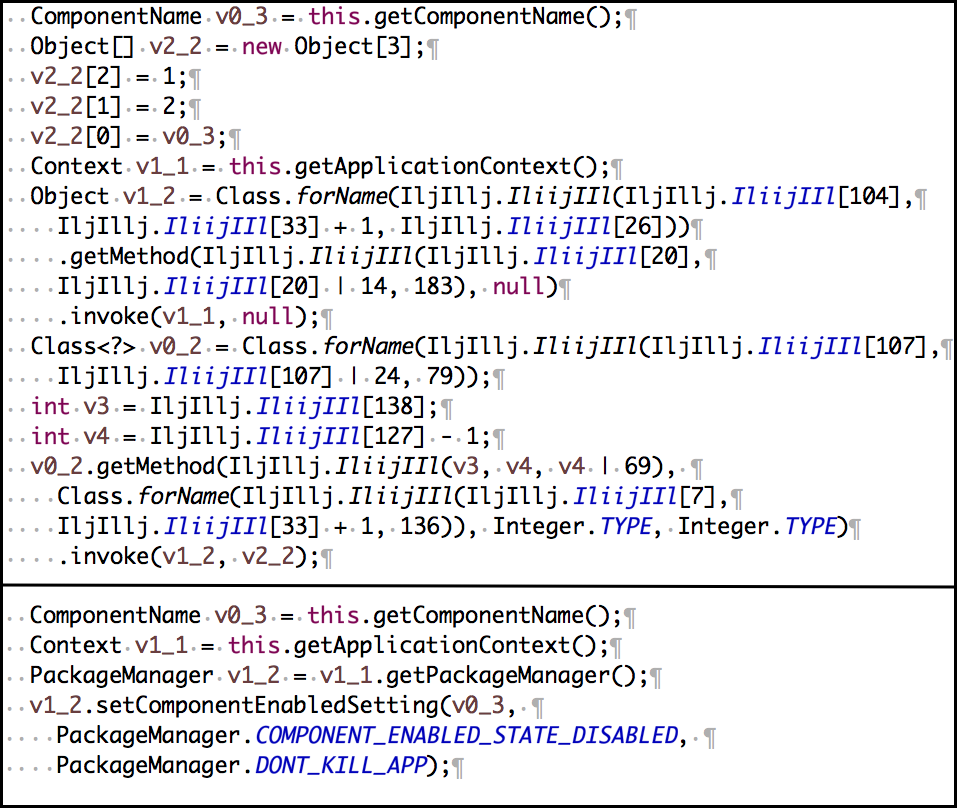
\includegraphics[width=3.5in]{fig/obadCodeSnippet.png}
\vspace{-.05in}
\caption{Obad Code Snippet. The obfuscated code is on the top; 
the de-obfuscated version is at the bottom.}
\label{fig:obadCodeSnippet}
\vspace{-.15in}
\end{figure}


One notable family that extensively adopts renaming and string encryption
techniques is \fn{Obad}.
Figure~\ref{fig:obadCodeSnippet} shows the code snippets
in \fn{Obad} and the corresponding translation.
We can see that, the obfuscation renames all classes, methods, fields to 
human unreadable forms (\eg {\em IljIllj}, {\em IliijIIl}, \etc).
Furthermore, all invoke statements
in the unobfuscated bytecode are translated to java reflection in the obfuscated version, 
and the name strings of such reflection are further encrypted and stored in a byte array 
list ``IliijIIl.''
The decrypting method ``{\em IljIllj.IliijIIl}'' takes the byte array from ``IliijIIl'' and
decrypts it and makes the reflection call.
This clearly shows that the obfuscation can make both manual analysis
and static analysis extremely difficult.

%\ptitle{Dynamic Loading (DL)}

{\bf Dynamic Loading} dex file becomes more popular nowadays. 
Normally it contains a dropper payload, which is lightweight
and looks benign.
But this dropper payload will then load the real
payload from its assets or resource folder (\eg \fn{RuMMS}), 
or download the real payload from internet (\eg \fn{SlemBunk}).
To further complicate the analysis, the real payload can even be encrypted (\eg \fn{Fobus}).

%\ptitle{Native Payload (NP)}

{\bf Native Payload}: Most of the static analysis tools focus on Dalvik bytecode.
So the native
library seems to be a good place to hide malware behavior.
In our analysis, we observed that native payloads are becoming
more popular. Malware apps not only hide functionalities,
but also hide sensitive strings, like server URL, premium numbers in the native code.
%\fn{xxx} hides the sms aborting logic in the native payload whereas
%\fn{Ogel} hides the url in the native payload.

%\ptitle{Evade Dynamic Analysis (EDA)}

% On the other hand, cybercriminals invented many ways to evade dynamic analysis.
{\bf Evade Dynamic Analysis}: The basic idea of evading dynamic analysis is to detect the malware's
current running environment.
For example,
when \fn{BankBot} \cite{bankBot} gets activated, it will check whether
IMEI, MODEL, FINGERPRINT, MANUFACTURE, BRAND and DEVICE are of certain
value.
%\begin{itemize}[noitemsep]
%\item Is {\em IMEI} equals ``000000000000000"?
%\item Is {\em Build.MODEL} contains ``google_sdk", ``Emulator", ``Android SDK", or ``Android SDK built for x86"?
%\item Is {\em Build.FINGERPRINT} starts with ``generic" or ``unknown"?
%\item Is {\em Build.MANUFACTURER}  contains ``Genymotion"?
%\item Is {\em Build.BRAND} starts with ``generic"?
%\item Is {\em Build.DEVICE} starts with ``generic"?
%\end{itemize}
If the running environment satisfies the condition,
it will act benignly and stop itself.
\fn{Triada} will check if IMEI matches some pattern, and
check whether ``com.qihoo. androidsandbox'' is installed.
To thwart dynamic analysis that monitors the communication
channel (\eg Internet, SMS.) of the malware,
many malware encrypt communication with their C\&C servers.

Many of these anti-analysis techniques involve encryption;
thus how to obtain the key is important to the analyst.
In most of the cases, the key is just hardcoded in the application code.
Some malware put the key in the
manifest, a resource XML file, or in the native payload.
We also observed a few smart ways to hide or generate the keys.
\fn{Fobus} reads the JVM stack trace and uses the class and method name
of the fourth entry in the stack to construct the key. 
\fn{Obad} obtains its key by requesting a webpage from Facebook, and reads
certain location from that webpage to generate the key.

%%% Local Variables: 
%%% mode: latex
%%% TeX-master: "paper"
%%% End: 
